\subsection{Exponential relationship between cell size and growth rate is
expected when growth is limited by ribosomal abundance.}

We next consider the consequences of our results on 
cell size and growth rate. The relationship between cell size and growth rate
has long been of interest in the study of bacteria, particularly following the
now decade-old observation that cell volume appears to increase exponentially
with growth rate; known as Schaechter's growth law  \citep{schaechter1958,
taheriaraghi2015}. Wild-type \textit{E. coli} growing at relatively fast growth
rates, show a remarkably constant cell cycle time ($t_cyc$, referring to the C +
D periods of DNA replication and cell division), as shown in \FIG{translation_ecoli_partA}(A) for the
data reproduced from \citep{si2017}. With a constant cell cycle time, the
exponential scaling has long been considered a direct consequence of cells
initiating replication at a constant volume per origin. However, the particular
mechanism that governs this relationship, and even the question of whether the
change in average cell size is truely exponental have remained under
debate \citep{si2017, harris2018}.

Under the simplest of strategies, for example, given the constraint set by
Equation 3 it would seem most appropriate for the cell to only adjust its
proteome through the synthesis of additional ribosomes. In contrast, it is clear
that a large portion of the proteome increases in absolute abundance. Cells
maintain a lineary scaling between size and number of origins that is robust to
a remarkable array of perturbations \citep{si2017}.  In\FIG{translation_ecoli_partA}(B) we show this
linear trend across the various proteomic data sets by estimating $\langle$\#
ori$\rangle$ from the measurements of \cite{si2017} for wild-type cells grown
under nutrient limitation. $\langle$\# ori$\rangle$ is determined by how often
replication forks must be initiated per cell cycle to maintain steady-state
growth, and is calculated from  2$^{\tau_{cyc} / \tau}$, where $\tau_{cyc}$.

Through our estimates in the preceeding sections on the central dogma, it is
apparent that the processes of transcription (i.e. synthesis of mRNA) and
translation are unlikely limiting steps in the process of doubling the
cell mass. This argues that as DNA replication beings to occur in parallel, the
proteome should only change in ways that reflect the change in DNA gene dosage
and the distribution of mRNA due to any additional aspects of gene regulation.
The total amount of protein synthesized over a cell cycle is nevertheless
determined by $R \times r_t \times \lambda$. Since protein accounts for most of
the cellular dry mass \citep{bremer2008, basan2015}, cell size will also vary
in proportional to this. The relationship between cell size and growth rate,
however, will ultimately depend only on how the cell varies its ribosomal
fraction, as highlighted by Equation 3.

It is notable that the majority of ribosomal proteins and rRNA operons are found
closer to the DNA origin. For relatively constant of $t_{cyc}$ and in
particular, the DNA replciation period $t_C$, parallelized DNA replication has
the important consequence in that it will skew absolute gene dosage and mRNA
abundance in favor of genes closer to the origin \citep{scholz2019} [more cites]
(\FIG{translation_ecoli_partA}(C)). This raises the possibility that for
moderately fast growth rates (above about 0.5 h$^{-1}$), the increased number of
replication forks can be viewed as a way for the cell to skew its ribosomal
abundance. Importantly, alternative solutions such as simply increases the
expression of ribsomes for a particular $\langle$\# ori$\rangle$ are not a
likely possibility if rRNA synthesis is nearly limiitng. This also provides a
means to maintain levels of expression for most other proteins needed  for
growth, which as we've seen throughout our estimates, also need to scale with
cell size. We were unaware, however, of whether such a skew gene dosage
materializes at the proteomic level. In order to see whether there is a relative
increase in protein expression for genes closer to the origin at faster growth,
we calculated a running boxcar average (500 kbp window) of protein copy number
as a function of each gene's transcriptional start site
(\FIG{translation_ecoli_partA}(D)). While absolute protein copy numbers can vary
substantially across the chromosome, we indeed observe a bias in expression
under fast growth conditions (dark blue). The dramatic change in protein copy
number near the origin is primarily due to the increase in ribosomal protein
expression. This trend is in contrast to slower growth conditions (yellow) where
the average copy number is more uniform across the length of the chromosome.

\begin{figure*}
    \begin{fullwidth}
    \centering{
        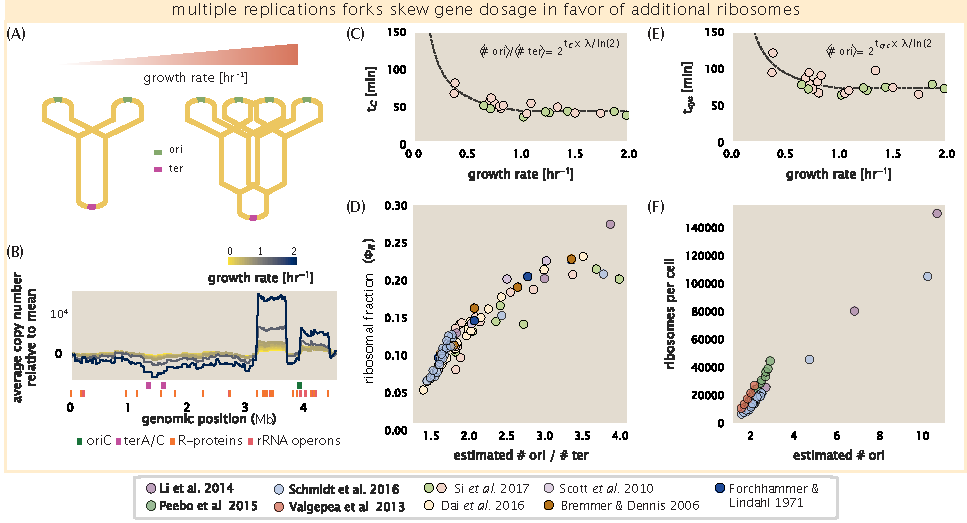
\includegraphics{main_figs/fig8_ribosome_growth_limit_ecoli_a.pdf}
        \caption{\textbf{Multiple replication forks skew gene dosage and
        ribosomal content.} (A) Experimental data from Si
        \textit{et al.} (2017). Dashed line shows fit to the data, which were
        used to estimate
        $\langle$\# ori$\rangle$. $t_cyc$ was assumed to vary in proportion to $tau$
        for doubling times great than 40 minutes, and then reach a minimum value of
        [fill in] minutes below this (see Supplemental Appendix X for additional details).
        Red data points
        correspond to measurements in strain MG1655, while light green points
        are for strain NCM3722.
        (B) Plot of the ribosome
        copy number estimated from the proteomic data against the estimated
        $\langle$\# ori$\rangle$ [NB: change to total protein abundance?].
        (C) Schematic shows the expected increase in
        replication forks (or number of ori regions) as \textit{E. coli} cells
        grow faster. (D) A running boxcar average of protein copy number is
        calculated for each each growth condition considered by Schmidt
        \textit{et al.}. A 0.5 Mb averaging window was used. Protein copy
        numbers are reported relative to their condition-specific means in order
        to center all data sets.
        (E)
        Experimental data from Si
        \textit{et al.} (2017) showing $t_C$ as a function of growth rate.
        Dashed line shows a best fit to the data, similar to part (A).
        (F) Plot compares our estimate of $\langle$\#
        ori$\rangle$ / $\langle$\# ter$\rangle$  to the experimental
        measurements of ribosomal abundance. Ribosomal fraction was approximated
        from the RNA/protein ratios of Dai \textit{et al.} (2016) (yellow) and
        Si \textit{et al.} (2017) (light red and light green) by the conversion
        RNA/protein ratio $\approx \Phi_R \cdot 2.1$. } \label{fig:translation_ecoli_partA}
    }
    \end{fullwidth}
\end{figure*}

%%%%%%%%%%%%%%%%%%%%%%%%
%%%%%%%%%%%%%%%%%%%%%%%%

%  It is only
% if ribosomal synthesis is rate limiting that the cell would need to vary
% [** As long as the cell maintains it's ability to synthesis ribosomes, i.e. not
% rate limiting, the cell will vary its ribosomal content according to number of origins
% it then follows  that cell size should scale with growth rate]
% ** However this breaks down when size  is not directly proportional to R.
% ***** It is only because R scales with number of origins that we get size vs. growth rate scaling.
% ***** (MAYBE) IF ribosomes are being synthesized in this regime essentially at their maximum amount,
% than it provides a possible explanation for the increase in ribosome abundance
%
%
% , albeit with a bias torward the origin of replication as discussed
% above. Indeed, most proteins exhibit a strong correlation with $\langle$\#
% ori$\rangle$, with the exception largely restricted to proteins involved in
% metabolism [make figure]. The total protein mass will then scale with
% $\langle$\# ori$\rangle$, which itself will be proportional to $R \times r_t
% \times \lambda$).
%
% Since size is largely determined by its protein and RNA mass, which account for
% over [70?] percent of total dry mass \citep{basan2015}, we can expect it to be
% proportional to the amount of protein synthesized over a cell cycle.  The
% specific scaling between $R$, and $\langle$\# ori$\rangle$, will depend on any
% growth dependent changes in both $r_t$ and any additional aspects of gene
% regulation. Nevertheless for an exponential increase in both $R$, and total
% protein content, there will be a linear increase in the ribosomal fraction
% $Phi_R$.  It then follows from Equation 2, that an increase in ribosomal
% fraction and proportionate increase in growth rate will be associated with an
% exponential increase in protein content and cell size.
%
% When ribosome synthesis is not rate limiting however, below about 0.5 hr$^{-1}$,
% ribosomal synthesis is no longer expected to be rate limiting and we
% have no reason to expect an exponential growth in size ?.
%
% %%%%%%%%%%%%%%%%%%%%%%%%%%%%
% %%%%%%%%%%%%%%%%%%%%%%%%%%%%

In the absence of gross global repression as $\langle$\# ori$\rangle$ increases,
we can then view a linear increase in $Phi_R$ (and $\lambda$) as requiring an increase
in total protein abundance that is proportional to $\langle$\# ori$\rangle$.
Initiation of chromosomal replication at fixed volume per origin then leads to an
exponential increase in total protein mass with growth rate $\lambda$.

\subsection{An exponential increase in chromosomal content provides diminishing
increases in growth rate.}

The ratio $\langle$\# ori$\rangle$ / $\langle$\# ter$\rangle$ can also be used
to consider the skew on chromosomal content. It will depends on how quickly
chromosomes are replicated (C period) relative the cell's doubling time $\tau$
and is given by 2$^{\tau_C / \tau}$. In \FIG{translation_ecoli_partA}(C) we plot
the measured $\tau_C$ versus $\tau$ (computed as $\tau = \log (2) / \lambda$)
from the wild-type \textit{E. coli} data of \citep{si2017}.  This is most
relevant to the ribosomal  fraction and in \FIG{translation_ecoli_partA}(D) we
plot the $\langle$\# ori$\rangle$ / $\langle$\# ter$\rangle$ ratio against
ribosomal fraction across a number of recent measurements.
% That work also measured the total RNA to protein ratio which
% reflects ribosomal abundance and we show that data along with other recent
% measurements from \cite{dai2016,dai2018}.
% Indeed, we find that the ribosomal
% fraction increases with $\langle$\# ori$\rangle$ / $\langle$\# ter$\rangle$
% (\FIG{translation_ecoli_partA}(C)). We note a systematic difference in the
% relative abundances from \cite{peebo2015} and \cite{valgepea2013} that was
% inconsistent with a number of other measurements of total RNA-to-protein ratios
% ($\approx \Phi_R$ x 2.1 \cite{dai2016}) and only show the data from
% \cite{schmidt2016} and \cite{li2014} for relative ribosome abundances (see
% supplemental section XX for a more complete discussion).
The ribosomal fraction doesn't increase as much at higher $\langle$\# ori$\rangle$ /
$\langle$\# ter$\rangle$. In part because rRNA operons are not all located
exactly,  there is likely a diminishing increase in ribosome abundance at higher
$\langle$\# ori$\rangle$ / $\langle$\# ter$\rangle$ ratios.

Importantly, however, the possibility that rRNA production is nearly rate limited, may
shed some light on some of the robust scaling between cell size  and
$\langle$\# ori$\rangle$. As one example, when cells are exposed to sublethal
doses of ribosome-inhibiting drugs like chloramphenicol, there is a notable
increase in the cell's ribosomal fraction \citep{scott2010, dai2016}. If rRNA
synthesis is essentially rate limited at these moderately  fast growth rates,
the presence of chloramphenicol should lengthen the doubling time and allow
increased rRNA synthesis relative to the rate of cell division. In Supplemental
Section XX, we consider this further using additional data from \cite{si2017}.


% Below growth rates of about 0.5 h$^{-1}$ it becomes less clear whether  two regimes where this scaling relationship is likely to falter: (1)
% slow growth, below about 0.5 hr$^{-1}$ where the number of ribosomes $R$ no
% longer reflects the number of actively translating ribosomes, and (2) ????
% fastest growth due to limits on rRNA production)

% \subsection{Maximizing growth rate requires coordination of biosynthesis at all growth rates.}
%
% However, the mechanism behind growth rate control has remained elusive
% and has only been described at a phenomenological level.
%
% Here we attempt to place our observations across the proteomic data sets in the
% context of \textit{E. coli} maximizing its steady-state growth rate across a wide
% array of conditions.

% \section{Parellel DNA replication biases protein production in support of ribosome synthesis.}
%
% \textit{E. coli} cells grow by a so-called "adder" mechanism, whereby cells add
% a constant volume with each cell division \citep{taheriaraghi2015}. In
% conjunction with this, additional rounds of DNA replication are triggered when
% cells reach a critical volume per origin of replication
% (\FIG{translation_ecoli_partA}(A)). This leads to the classically-described
% exponential increase in cell size with growth rate \cite{schaechter1958, si2017,
% si2019}. In the context of maximizing growth rate, it is notable that the
% majority of ribosomal proteins and rRNA operons are found closer to the DNA
% origin.

% Given that cells must
% increase their total gene dosage of rRNA operons at faster growth rates, and the
% intimate relationship between ribosomal content and growth rate considered
% above, this raises the possibility that the increase in chromosomal content
% might simply be a means for the cell to tune biosynthesis according to its
% physiological state and the nutrient availability in its environment.

% While an increase in transcription has been observed for genes closer to the
% origin in rapidly growing \textit{E. coli} \citep{scholz2019}, we were unaware
% of such characterization at the proteomic level. In order to see whether there
% is a relative increase in protein expression for genes closer to the origin at
% faster growth, we calculated a running boxcar average (500 kbp window) of
% protein copy number as a function of each gene's transcriptional start site
% (\FIG{translation_ecoli_partA}(B)). While absolute protein copy numbers can vary
% substantially across the chromosome, we indeed observe a bias in expression
% under fast growth conditions (dark blue). The dramatic change in protein copy
% number near the origin is primarily due to the increase in ribosomal protein
% expression. This trend is in contrast to slower growth conditions (yellow) where
% the average copy number is more uniform across the length of the chromosome.
%
% \begin{figure*}
%     \begin{fullwidth}
%     \centering{
%         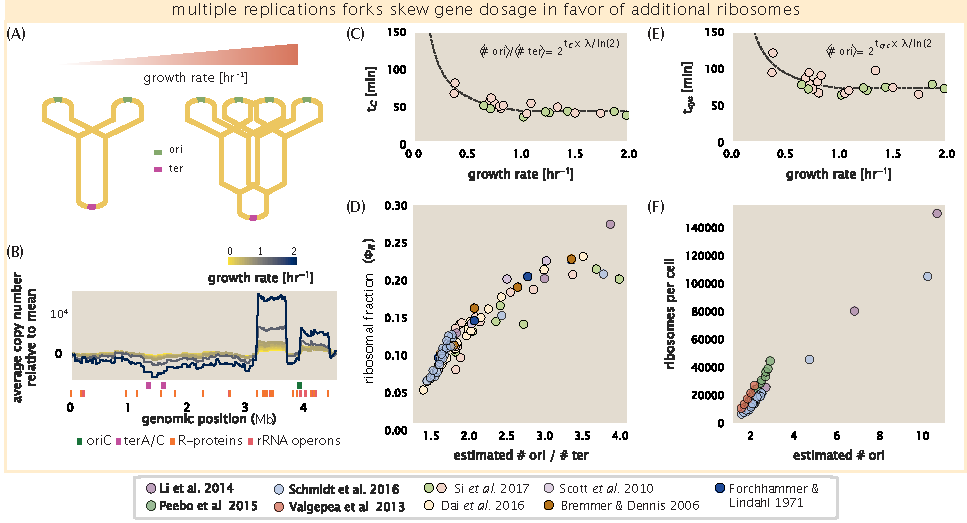
\includegraphics{main_figs/fig8_ribosome_growth_limit_ecoli_a.pdf}
%         \caption{\textbf{Multiple replication forks skew gene dosage and
%         ribosomal content.} (A) Schematic shows the expected increase in
%         replication forks (or number of ori regions) as \textit{E. coli} cells
%         grow faster. (B) A running boxcar average of protein copy number is
%         calculated for each each growth condition considered by Schmidt
%         \textit{et al.}. A 0.5 Mb averaging window was used. Protein copy
%         numbers are reported relative to their condition-specific means in order
%         to center all data sets. (C) and (E) show experimental data from Si
%         \textit{et al.} (2017) Solid lines show fits to the data, which were
%         used to estimate $\langle$\# ori$\rangle$ / $\langle$\# ter$\rangle$ and
%         $\langle$\# ori$\rangle$ [NB: to note fit equations]. Red data points
%         correspond to measurements in strain MG1655, while light green points
%         are for strain NCM3722. (D) Plot compares our estimate of $\langle$\#
%         ori$\rangle$ / $\langle$\# ter$\rangle$  to the experimental
%         measurements of ribosomal abundance. Ribosomal fraction was approximated
%         from the RNA/protein ratios of Dai \textit{et al.} (2016) (yellow) and
%         Si \textit{et al.} (2017) (light red and light green) by the conversion
%         RNA/protein ratio $\approx \Phi_R \cdot 2.1$. (F) Plot of the ribosome
%         copy number estimated from the proteomic data against the estimated
%         $\langle$\# ori$\rangle$.} \label{fig:translation_ecoli_partA}
%     }
%     \end{fullwidth}
% \end{figure*}

% \subsection{Ribosome abundance increases in proportion to expected rRNA gene dosage.}
%
% If ribosomal genes (rRNA and ribosomal proteins) are growth rate limiting and
% synthesized according to the available rRNA gene
% dosage and condition-dependent transcription rate, we expect that ribosomal
% abundance will vary in proportion to the increase in rRNA gene dosage. This will be related to $\langle$\# ori$\rangle$ and the $\langle$\# ori$\rangle$ /
% $\langle$\# ter$\rangle$ ratio.

% To estimate rRNA gene dosage, we considered the experimental data
% from \cite{si2017}, which inferred these parameters for cells under
% nutrient-limited growth. The ratio $\langle$\# ori$\rangle$ / $\langle$\#
% ter$\rangle$ depends on how quickly chromosomes are replicated relative the
% cell's doubling time $\tau$ and is given by 2$^{\tau_C / \tau}$. Here $\tau_C$
% is the time taken to replicate \textit{E. coli}'s chromosome, referred to as the
% C period of cell division.  In \FIG{translation_ecoli_partA}(C) we plot the
% measured $\tau_C$ versus $\tau$ (computed as $\tau = \log (2) / \lambda$), with
% data points in red corresponding to \textit{E. coli} strain MG1655, and blue to
% strain NCM3722. \cite{si2017} also measured the total RNA to protein ratio which
% reflects ribosomal abundance and we show that data along with other recent
% measurements from \cite{dai2016,dai2018}. Indeed, we find that the ribosomal
% fraction increases with $\langle$\# ori$\rangle$ / $\langle$\# ter$\rangle$
% (\FIG{translation_ecoli_partA}(C)). We note a systematic difference in the
% relative abundances from \cite{peebo2015} and \cite{valgepea2013} that was
% inconsistent with a number of other measurements of total RNA-to-protein ratios
% ($\approx \Phi_R$ x 2.1 \cite{dai2016}) and only show the data from
% \cite{schmidt2016} and \cite{li2014} for relative ribosome abundances (see
% supplemental section XX for a more complete discussion). For the data shown, the
% ribosomal fraction doesn't increase as much at higher $\langle$\# ori$\rangle$ /
% $\langle$\# ter$\rangle$. Since several rRNA operons are actually located
% approximately half-way between the origin and terminus, the trend may in part be
% a consequence of a diminishing increase in rRNA gene dosage at higher
% $\langle$\# ori$\rangle$ / $\langle$\# ter$\rangle$ ratios.


% protein fraction should
% increase in proportion to the average ratio of DNA origins to DNA termini
% ($\langle$\# ori$\rangle$ / $\langle$\# ter$\rangle$ ratio).

% we can make two related hypotheses about how their ribosome abundance should
% vary with chromosomal content. First, the ribosomal protein fraction should
% increase in proportion to the average ratio of DNA origins to DNA termini
% ($\langle$\# ori$\rangle$ / $\langle$\# ter$\rangle$ ratio). This is a
% consequence of the skew in DNA dosage as cells grow faster. The second
% hypothesis is that the absolute number of ribosomes should increase with the
% number of DNA origins ($\langle$\# ori$\rangle$), since this will reflect the
% total gene dosage at a particular growth condition.


% We can similarly estimate $\langle$\# ori$\rangle$, which depends on how often
% replication forks are initiated per cell cycle. This is given by the number of
% overlapping cell cycles,  2$^{\tau_{cyc} / \tau}$, where $\tau_{cyc}$, refers to
% the total time of chromosome replication and cell division.
% \FIG{translation_ecoli_partA}(E) shows the associated data from \cite{si2019},
% which we use to estimate $\langle$\# ori$\rangle$  for each growth condition of
% the proteomic data. In agreement with our expectations, we find that ribosome
% copy number increases with the estimated $\langle$\# ori$\rangle$
% (\FIG{translation_ecoli_partA}(F)).



% While it is difficult to distinguish between causality and correlation, the data
% also helps us resolve why cell size, should exhibit an exponential increase with growth
% rate once cells begin to parallelize DNA replication. Specifically,
%
% is consistent with the need for cells to increase their effective rRNA gene
% dosage in order to grow according to the constraint set by Equation 2. Importantly, it
% may also shed some light on the notable increase in ribosomal content
% that is observed when sublethal doses of antibiotics \citep{scott2010, dai2016}.
% Specifically, if rRNA synthesis is rate limiting, and nutrient conditions
% largely dictate the extent of overlapping DNA replication cycles, than addition
% of antibiotic will lengthen the doubling time and allow increased rRNA
% synthesis relative to the rate of cell division. In Supplemental Section XX, we
% consider this further using additional data from \cite{si2017}.

\section{Mitigation of biosynthesis helps maintain maximal steady-state growth
in poor nutrient conditions.}

While the above observations show how \textit{E. coli} point to a role by
ribsomes in setting the exponential growth in cell size, this relationship is
likely to falter at slow growth rates where it has become apparent that $R$ is
no longer a direct reflection of protein synthesis capacity \citep{dai2016}.
% Specifically, here we consider the recent obser
 % vary its ribosomal
% content to increase growth rate, it also presents a challenge in the limit of
% poorer nutrient conditions.
Recall from Equation \ref{eq:translation_limit_growth_rate} that ribosomal
content should decrease to zero as growth decreases to zero. While bacteria tend
to decrease their ribosomal abundance in poorer nutrient conditions, they do so
only to some fixed, non-zero amount \citep{scott2010, liebermeister2014}. Here
we find a minimal ribosomal fraction of $\approx$ 0.06 in the slowest growth
conditions. From the perspective of a bacterium dealing with uncertain nutrient
conditions, there is likely a benefit for the cell to maintain some relative
fraction of ribosomes to support rapid growth as nutrient conditions improve.

The challenge then for cells at slow growth, lies in their ability to maintain growth when
ribosomes are in excess of the rate that nutrients can be harvested \FIG{translation_ecoli_partB}{A}. Ribosomes would consume their amino acid supply and
be unable to maintain steady-state growth in sufficiently poor nutrient conditions. In reality, \textit{E. coli} is still
able to maintain a relatively high elongation rate even in stationary phase
($\approx$ 8 AA/s, \citep{dai2016, dai2018}). A explanation for this is that the
cell further regulates its biological activity in conditions of stress and
nutrient-limitation; in particular through the small-molecule alarmones (p)ppGpp
\citep{harris2018}. In (p)ppGpp null strains, cells are unable to grow in
nutrient-poor media. Indeed, these small molecules play a role in controlling
biosynthesis rates throughout the central dogma [NB citations]. Here we explore
this further in the context of protein synthesis.

Under slow growth conditions ($\lambda$ less than \~ 0.5 $hr^{-1}$) we assume
that the reported decrease in elongation rate is due to a limiting supply of
amino acids. We proceed by coarse graining the cell's amino acid supply as an
single, effective rate-limiting species (see Supplmental Section XX for a more
complete discussion). Under such a scenario, the elongation rate can described
as simply depending on the maximum elongation rate ($\approx$ 17.1 aa/s,
\citep{dai2016, dai2018}), an effective $K_d$, and the limiting amino acid
concentration $[AA]_{eff}$. Specifically, the elongation rate is given by,

\begin{equation}
r_t = r_t^{max} \cdot \frac{1}{1 + K_d / [AA]_{eff}}.
\label{eq:rate_Kd}
\end{equation}
For cells growing in minimal media + glucose, the amino acid concentration is of
order 100 mM  (BNID: 110093, \citep{milo2010, bennett2009}). With a growth rate
of about 0.6 hr$^{-1}$ and elongation rate of 12.5 aa per second
\citep{dai2016}, we can estimate an effective $K_d$ of about 40 mM. Ultimately
the steady state amino acid concentration will depend on the difference between
the supply of amino acids $r_{aa}$ and consumption by ribosomes $r_t \cdot R
\cdot f_a$, where $f_a$ accounts for the possible reduction of actively
translating ribosomes.

In \FIG{translation_ecoli_partB}{B} we consider how the maximal growth rates and
elongation rates vary as a function of the number of actively translating
ribosomes in this slow growth regime (see Supplemental Section XX for a complete
description of this model). If we consider $r_{AA}$ to be reflective of a
specific growth condition (dashed lines), cells grow fastest by maximizing their
fraction of actively translating ribosomes. When we consider the experimental
measurements from \cite{dai2018} (yellow circles), which reflect growth in
different nutrient conditions, we see that cells reduce $R \times f_a$ in poorer
nutrient conditions, but in a way that keeps $[AA]_{eff}$ relatively constant.
Given our estimate for the $K_d$ of 40 mM,  we would only expect a decrease from
100 mM to about 35 mM in the slowest growth conditions. While experimental data
is limited, amino acid concentrations only decrease to about 60 mM for cells
grown in minimal media + acetate ($\lambda$ ~ 0.3 hr$^{-1}$ in our proteomic
data; concentration obtained from \cite{bennett2009}), qualitatively consistent
with our expectations.  One explanation for this is that the cell needs to
maintain a sufficiently  high pool of amino acids to maintain steady-state
growth. Any further increase in $R \times f_a$ at constant $r_{AA}$ would be
associated with a further drop in cellular amino acids concentrations.


\begin{figure*}
    \begin{fullwidth}
    \centering{
        \includegraphics{main_figs/fig8_ribosome_growth_limit_ecoli_b.pdf}
        \caption{\textbf{\textit{E. coli} must regulate ribosomal activity in
        limiting nutrient conditions. }
        (A) Schematic showing translation-specific requirements for maintenance
        of steady-state growth. In a nutrient rich environment, amino acid
        supply $r_{aa}$ is sufficiently in excess of the demand by ribosomes
        translating at their maximal rate. In poorer nutrient conditions,
        reduced amino acid supply $r_{aa}$ will decrease the rate of elongation.
        In a regime where $r_{aa}$ is less than $r_t \cdot R$, the number of
        actively translating ribosomes will need to be reduced in order to
        maintain steady-state growth. (B) Translation elongation rate is plotted
        as a function of the number of actively translating ribosomes $R \cdot
        f_a$. Dashed lines correspond to a range of amino acid synthesis rates
        $r_{aa}$, from 10$^3$ to 10$^6$. Growth rates are calculated according
        to Equation 1, assuming a constant ribosomal fraction of 8 percent. See
        appendix XX for additional details. (C) Experimental data from Dai
        \textit{et al.} are used to estimate the fraction of actively
        translating ribosomes. The solid line represents the translation-limited
        growth rate for ribosomes elongating at 17.1 AA/s. }
        \label{fig:translation_ecoli_partB}
    }
    \end{fullwidth}
\end{figure*}

Using the quantitative data from \cite{dai2018}, which determined $f_a$ across
the entire range of growth rates across our data, we next estimated the active
fraction of ribosomal protein. As shown in \FIG{translation_ecoli_partB}(C), we
find that cells grow at a rate near the expected translation maximum expected
from Equation 1, using the maximum elongation rate of $r_t$ = 17.1 aa per
second. This is in contrast to the reality that ribosomes are translating at
almost half this rate in the poorest growth conditions.  Specifically, here it
is by adjusting $r_t \times R \times f_a$ that cells are able to maximize their
growth rate across a vast range of growth conditions.


%
% \subsubsection{Global regulatory control across central dogma may
% provide an explanation for the robust scaling laws in \textit{E. coli}.}
